\begin{frame}
    \frametitle{Representación de pose en 2D}
    \footnotesize
    Modelamos el robot como un cuerpo rígido sobre ruedas, que opera en un plano horizontal. La dimensionalidad total de este chasis de robot en el plano es de tres, dos para la posición en el plano y uno para la orientación a lo largo del eje vertical, que es ortogonal al plano.

    \begin{figure}[!h]
        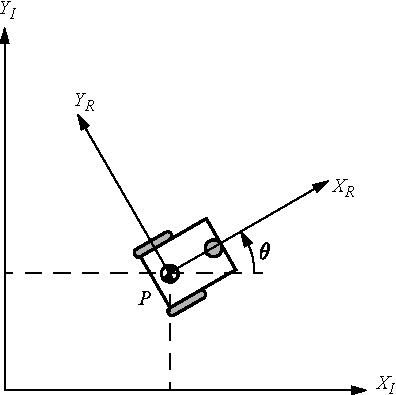
\includegraphics[width=0.4\columnwidth]{./images/coordinate_systems.pdf}
        \caption{El marco de referencia global y el marco de referencia local del robot.}
    \end{figure}

    Para especificar la posición del robot en el plano, establecemos una relación entre el marco de referencia global y el marco de referencia local del robot.

\end{frame}


\begin{frame}
    \frametitle{Representación de pose en 2D}
    \footnotesize

    \begin{center}
        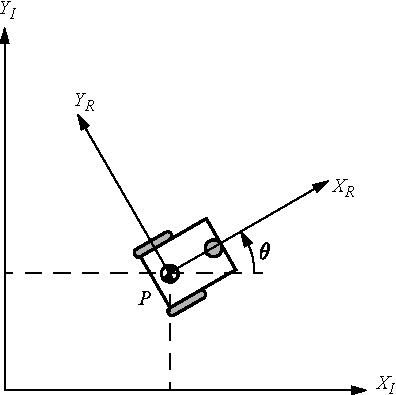
\includegraphics[width=0.4\columnwidth]{./images/coordinate_systems.pdf}
    \end{center}

    \note{Un marco de referencia inercial es un marco de referencia que no está experimentando aceleración. La física de un sistema en un marco inercial no tiene fuerzas externas al sistema.}

    \note{Ejemplo de sistema no inercial: una bola que cae hacia el suelo no va exactamente hacia abajo porque la Tierra está girando, lo que significa que el marco de referencia de un observador en la Tierra no es inercial. La física debe tener en cuenta el efecto Coriolis, en este caso considerado como una fuerza, para predecir el movimiento horizontal.}


    Para especificar la posición del robot, elegimos un punto $p$ en el chasis del robot como su punto de referencia de posición. La base $\left\lbrace X_R,Y_R \right\rbrace$ define dos ejes en relación con $p$ en el chasis del robot y, por lo tanto, es el marco de referencia local del robot. La posición de $p$ en el marco de referencia global se especifica mediante las coordenadas $x$ e $y$, y la diferencia angular entre los marcos de referencia global y local está dada por $\theta$.

    La pose del robot estará dada por la posición y la orientación:

    \begin{equation*}
        \xi_{I} = \begin{bmatrix}
            x\\
            y\\
            \theta
        \end{bmatrix}
    \end{equation*}
\end{frame}

\begin{frame}
    \frametitle{Traslación en 2D}
    \begin{equation*}
        {\displaystyle {\begin{bmatrix}x'\\y'\\\end{bmatrix}}={\begin{bmatrix} x\\y\end{bmatrix}}+{\begin{bmatrix}t_x\\t_y\\\end{bmatrix}}.}
    \end{equation*}
\end{frame}

\begin{frame}
    \frametitle{Rotación en 2D}
    \begin{equation*}
        {\displaystyle R(\theta )={\begin{bmatrix}\cos \theta &-\sin \theta \\\sin \theta &\cos \theta \\\end{bmatrix}}.}
    \end{equation*}

    \begin{equation*}
        {\displaystyle {\begin{bmatrix}x'\\y'\\\end{bmatrix}}={\begin{bmatrix}\cos \theta &-\sin \theta \\\sin \theta &\cos \theta \\\end{bmatrix}}{\begin{bmatrix}x\\y\\\end{bmatrix}}.}
    \end{equation*}

    \begin{equation*}
        {\displaystyle {\begin{aligned}x'&=x\cos \theta -y\sin \theta \,\\y'&=x\sin \theta +y\cos \theta \,\end{aligned}}.}
    \end{equation*}

\end{frame}


\begin{frame}
    \frametitle{Rototraslación en 2D}

    \begin{equation*}
        {\displaystyle {\begin{bmatrix}x'\\y'\\\end{bmatrix}}={\begin{bmatrix}\cos \theta &-\sin \theta \\\sin \theta &\cos \theta \\\end{bmatrix}}{\begin{bmatrix}x\\y\\\end{bmatrix}}+{\begin{bmatrix}t_x\\t_y\\\end{bmatrix}}.}
    \end{equation*}

    \begin{equation*}
        {\displaystyle {\begin{bmatrix}x'\\y'\\\end{bmatrix}}={R(\theta )\begin{bmatrix} x\\y\end{bmatrix}}+ \vec{t}.}
    \end{equation*}
\end{frame}


\begin{frame}
    \frametitle{Rotación en 3D}
    \small
    \begin{equation*}
        {\displaystyle {\begin{alignedat}{1}R_{x}(\theta )&={\begin{bmatrix}1&0&0\\0&\cos \theta &-\sin \theta \\[3pt]0&\sin \theta     &\cos \theta \\[3pt]\end{bmatrix}}\\
        R_{y}(\theta )&={\begin{bmatrix}\cos \theta &0&\sin \theta \\[3pt]0&1&0\\[3pt]-\sin \theta &0&\cos \theta \\
        \end{bmatrix}}\\
        R_{z}(\theta )&={\begin{bmatrix}\cos \theta &-\sin \theta &0\\[3pt]\sin \theta &\cos \theta &0\\[3pt]0&0&1\\\end{bmatrix}}\end{alignedat}}
        }
    \end{equation*}

Ejemplo:
    \begin{equation*}
        {\displaystyle R_{z}(90^{\circ }){\begin{bmatrix}1\\0\\0\\\end{bmatrix}}={\begin{bmatrix}\cos 90^{\circ }&-\sin 90^{\circ }&0\\\sin 90^{\circ }&\quad \cos 90^{\circ }&0\\0&0&1\\\end{bmatrix}}{\begin{bmatrix}1\\0\\0\\\end{bmatrix}}={\begin{bmatrix}0&-1&0\\1&0&0\\0&0&1\\\end{bmatrix}}{\begin{bmatrix}1\\0\\0\\\end{bmatrix}}={\begin{bmatrix}0\\1\\0\\\end{bmatrix}}}
    \end{equation*}

\end{frame}

\begin{frame}
    \frametitle{Rotaciones generales 3D}
    \tiny
    Rotación intrínseca con ángulos yaw, pitch y roll como $\alpha$, $\beta$ y $\gamma$. Formalmente, es una rotación intrínseca con ángulos Tait–Bryan angles $\alpha$, $\beta$ y $\gamma$ sobre los ejes $z$, $y$, $x$.
    \begin{equation*}
        {\displaystyle {\begin{aligned}R=R_{z}(\alpha )\,R_{y}(\beta )\,R_{x}(\gamma )&={\overset {\text{yaw}}{\begin{bmatrix}\cos \alpha &-\sin \alpha &0\\\sin \alpha &\cos \alpha &0\\0&0&1\\\end{bmatrix}}}{\overset {\text{pitch}}{\begin{bmatrix}\cos \beta &0&\sin \beta \\0&1&0\\-\sin \beta &0&\cos \beta \\\end{bmatrix}}}{\overset {\text{roll}}{\begin{bmatrix}1&0&0\\0&\cos \gamma &-\sin \gamma \\0&\sin \gamma &\cos \gamma \\\end{bmatrix}}}\\&={\begin{bmatrix}\cos \alpha \cos \beta &\cos \alpha \sin \beta \sin \gamma -\sin \alpha \cos \gamma &\cos \alpha \sin \beta \cos \gamma +\sin \alpha \sin \gamma \\\sin \alpha \cos \beta &\sin \alpha \sin \beta \sin \gamma +\cos \alpha \cos \gamma &\sin \alpha \sin \beta \cos \gamma -\cos \alpha \sin \gamma \\-\sin \beta &\cos \beta \sin \gamma &\cos \beta \cos \gamma \\\end{bmatrix}}\end{aligned}}}
    \end{equation*}
     De manera similar rotación extínseca con ángulos de Euler $\alpha$, $\beta$ y $\gamma$ sobre los ejes $x$, $y$ y $z$.
    \begin{equation*}
        {\displaystyle R=R_{z}(\gamma )\,R_{y}(\beta )\,R_{x}(\alpha )={\begin{bmatrix}\cos \gamma &-\sin \gamma &0\\\sin \gamma &\cos \gamma &0\\0&0&1\\\end{bmatrix}}{\begin{bmatrix}\cos \beta &0&\sin \beta \\0&1&0\\-\sin \beta &0&\cos \beta \\\end{bmatrix}}{\begin{bmatrix}1&0&0\\0&\cos \alpha &-\sin \alpha \\0&\sin \alpha &\cos \alpha \\\end{bmatrix}}}
    \end{equation*}

\end{frame}


\begin{frame}
    \frametitle{Propiedades de matrices Rotación en 3D}
    \small
    \begin{itemize}
        \item ${\displaystyle R^{\mathsf {T}}=R^{-1}}$ Matriz ortogonal
        \item $\det R = \pm 1$
    \end{itemize}

    Determinar el ángulo de una matriz de rotación utilizando la traza de la matriz (la suma de los elementos de la diagonal del matriz).
    \begin{equation*}
        {\displaystyle \operatorname {tr} (R)=1+2\cos \theta ,}
    \end{equation*}

    \begin{equation*}
        {\displaystyle |\theta |=\arccos \left({\frac {\operatorname {tr} (R)-1}{2}}\right).}
    \end{equation*}

\end{frame}

\begin{frame}
    \frametitle{Rotación representada con Axis-angle}
    La notación axial-angular es equivalente al más conciso vector de rotación, también llamado vector de Euler. En este caso, tanto el eje de rotación como el ángulo están representados por un vector codireccional con el eje de rotación cuyo módulo (longitud) coincide con el ángulo de rotación $\theta$,
    \begin{center}
        \begin{minipage}{0.38\linewidth}
        \small
        \begin{equation*}
            {\displaystyle {\boldsymbol {\theta }}=\theta \mathbf {e} \,.}
        \end{equation*}
        \begin{equation*}
            {\displaystyle (\mathrm {eje} ,\mathrm {\text{ángulo}} )=\left({\begin{bmatrix}e_{x}\\e_{y}\\e_{z}\end{bmatrix}},\theta \right)}
        \end{equation*}
        \end{minipage}
        \hspace{1em}
        \begin{minipage}{0.38\linewidth}
            \centering
            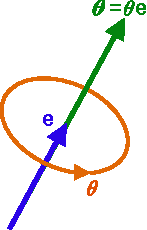
\includegraphics[width=0.5\columnwidth]{images/axis_angle_vector.pdf}
        \end{minipage}
    \end{center}

Ejemplo un vector de rotación con una magnitud de $\dfrac{\pi}{2}$ apuntando en la dirección $z$:
    \begin{equation*}
        {\displaystyle {\left({\begin{bmatrix}0\\0\\1\end{bmatrix}},{\frac {\pi }{2}}\right) = \begin{bmatrix}0\\0\\{\frac {\pi }{2}}\end{bmatrix}}.}
    \end{equation*}

    \note{The representation is very intuitive, but for actually applying the rotation, another representation is required, such as a quaternion or rotation matrix.}

\end{frame}

\begin{frame}
    \frametitle{Quaternions}
    Los cuaterniones es una generalización de números complejos con tres números imaginarios (i, j y k). Es un número complejo de cuatro dimensiones que se puede utilizar para representar la orientación de un cuerpo rígido o un marco de coordenadas en un espacio tridimensional. La definición general de un cuaternión viene dada por:
    %
    \begin{equation*}
        q = w + q_x i + q_y j + q_z k = \begin{bmatrix} q_w & q_x & q_y & q_z\end{bmatrix}
    \end{equation*}

    Los cuaterniones representan una transformación de rotación en 3D. Por lo tanto, la forma más fácil de representar un cuaternión es imaginar la rotación de un ángulo dado alrededor de un vector dado. La siguiente figura ilustra la rotación del ángulo $\theta$ alrededor del vector $\vec{v} = [v_{x} v_{y} v_{z}]$. El cuaternión asociado a esta rotación está dado por:
    %
    \begin{align*}
        q &= \begin{bmatrix} q_w & q_x & q_y & q_z\end{bmatrix}\\
        q &= \begin{bmatrix}
            \cos \frac{\theta}{2} & v_{x} \sin \frac{\theta}{2} & v_{y} \sin \frac{\theta}{2} & v_{z}\sin \frac{\theta}{2}
            \end{bmatrix}
    \end{align*}

\end{frame}

\begin{frame}
    \frametitle{Representación de pose en 2D}
    \footnotesize

    \begin{center}
        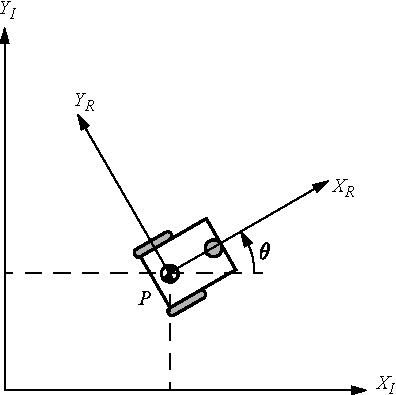
\includegraphics[width=0.4\columnwidth]{./images/coordinate_systems.pdf}
    \end{center}

    Esta matriz se puede utilizar para mapear el movimiento en el marco de referencia global ?? XI YI? al movimiento en términos del marco de referencia local ?? XR YR ?. Esta operación se denota por R? ()? ·

    \begin{equation*}
        R(\theta)=\begin{bmatrix}
            \cos\theta & \sin\theta & 0\\
            -\sin \theta & \cos \theta & 0\\
            0 & 0 & 1
        \end{bmatrix}
    \end{equation*}

    \begin{equation*}
        \dot{\xi_R} = R(\dfrac{\pi}{2}) \dot{\xi_I}
    \end{equation*}

    Dada alguna velocidad (??? · X · y ·) en el marco de referencia global, podemos calcular las componentes del movimiento a lo largo de los ejes locales XR y de este robot. En este caso, debido al ángulo YR específico del robot, el movimiento a lo largo de XR es igual a, y el movimiento a lo largo de YR es: y · –x ·

\end{frame}

\begin{frame}
    \frametitle{Right-hand rule}
    En Robótica la disposición de los ejes de coordenadas y el sentido de rotación de los mismos está dado por la regla de la mano derecha (Right-hand rule).

    \begin{figure}[!h]
        \centering
        \subfloat[]
        {
            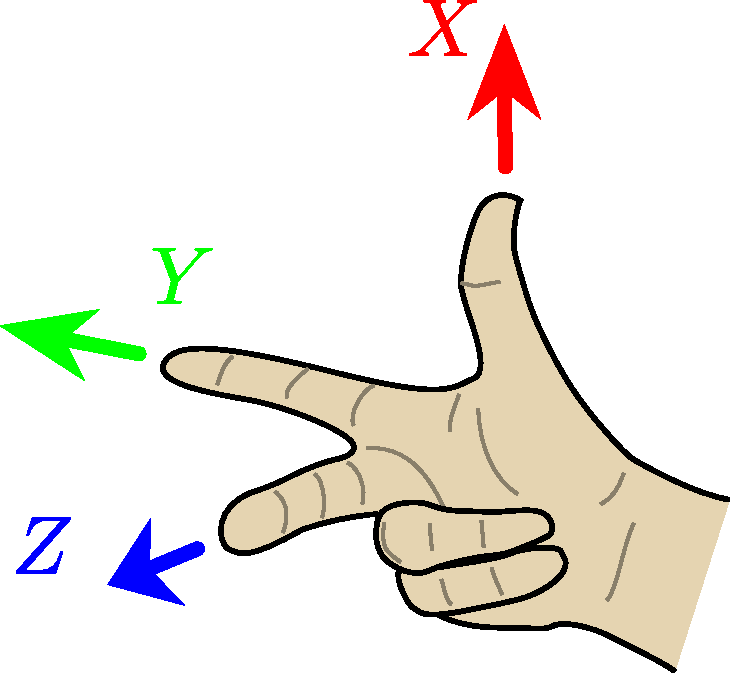
\includegraphics[width=0.4\columnwidth]{./images/right_hand_rule.pdf}
        }\hfill
        \subfloat[]
        {
            
\includegraphics[width=0.4\columnwidth]{./images/right_hand_rule_positive_rotation.pdf}
        }
    \end{figure}
\end{frame}

\begin{frame}
    \frametitle{Roll Pitch Yaw }
        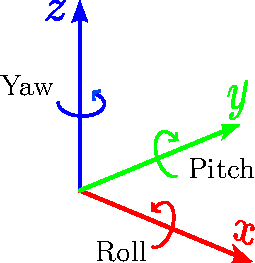
\includegraphics[width=0.5\columnwidth]{./images/roll_pitch_yaw.pdf}

        \TODO{Gimbal-Lock Video explanation: https://youtu.be/-WXfEPg8eMM}
\end{frame}

\begin{frame}
    \frametitle{Left-hand vs Right-hand rule}
    \begin{center}
        \only<1>{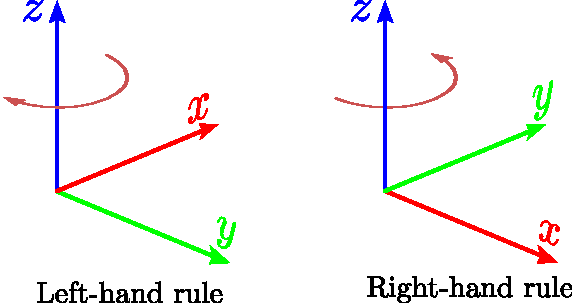
\includegraphics[width=\columnwidth]{./images/left_right_hand_rule.pdf}}
        \only<2>{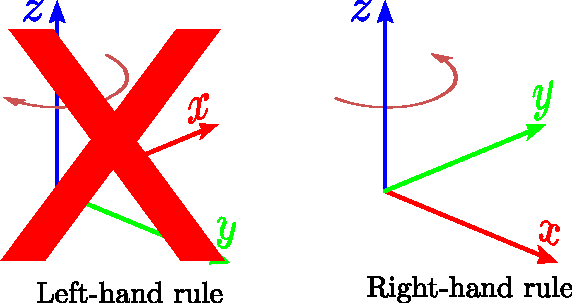
\includegraphics[width=\columnwidth]{./images/left_right_hand_rule_cross.pdf}}
    \end{center}
\end{frame}

\begin{frame}
    \TODO{Crear una práctica donde los chicos jueguen con traslaciones, rotaciones transformaciones. Quaterniones.}
\end{frame}
